% !TeX spellcheck = en_US
\documentclass[aspectratio=1610]{beamer}
\usetheme{Madrid}
\setbeamercovered{transparent}
\setbeamertemplate{navigation symbols}{}
\setbeamertemplate{itemize items}[circle]
\setbeamertemplate{enumerate items}[default]

\makeatletter
\define@key{beamerframe}{wide}[10pt]{%
	\def\beamer@cramped{\itemsep #1\topsep0.5pt\relax}}
\makeatother
	

\usepackage[english]{babel}
\usepackage[utf8]{inputenc}
\usepackage[T1]{fontenc}
\usepackage{array}
\usepackage{xcolor}
\usepackage{colortbl}
\usepackage{booktabs}

\title[Winter - Lecture 9] % (optional, use only with long paper titles)
{Intermediate Macroeconomics: Lecture  W9 (Ch.15)}
\subtitle{ECON 311 -- Intermediate Macroeconomics}

\author{Muhebullah Karimzada}
\institute{School of Economics \\\ University of Northern British Columbia}
\date{Fall 2026}


% ---------- UNBC COLORS ----------
\usepackage{xcolor}
\definecolor{UNBCGreen}{RGB}{0,102,51}
\definecolor{UNBCDark}{RGB}{0,74,37}
\definecolor{UNBCGold}{RGB}{189,155,96}
\definecolor{SoftCream}{RGB}{249,247,242}
\definecolor{SoftGray}{RGB}{244,246,248}
\definecolor{AccentBlue}{RGB}{41,98,255}
\definecolor{AccentOrange}{RGB}{230,126,34}
\definecolor{AccentTeal}{RGB}{0,150,136}
\definecolor{AccentRed}{RGB}{192,57,43}
\setbeamercolor{normal text}{fg=black,bg=white}
\setbeamercolor{structure}{fg=UNBCDark}
\setbeamercolor{title}{fg=white,bg=UNBCDark}
\setbeamercolor{subtitle}{fg=UNBCGold}
\setbeamercolor{frametitle}{fg=white,bg=UNBCDark}
\setbeamercolor{block title}{fg=white,bg=UNBCDark}
\setbeamercolor{block body}{fg=black,bg=SoftGray}
\setbeamercolor{block title alerted}{fg=white,bg=AccentRed}
\setbeamercolor{block body alerted}{fg=black,bg=SoftGray}
\setbeamercolor{item}{fg=UNBCDark}
\setbeamercolor{section in toc}{fg=UNBCDark}
\setbeamercolor{alerted text}{fg=AccentRed}
\setbeamercolor{author in head/foot}{fg=white,bg=UNBCDark}
\setbeamercolor{date in head/foot}{fg=white,bg=UNBCDark}
% ---------- UNBC BRANDING ----------
\usepackage{graphicx}
\usepackage{lmodern}
\usepackage{tcolorbox}
\usepackage{tikz}
\usetikzlibrary{positioning,calc}
\setbeamertemplate{headline}{}
\setbeamertemplate{footline}{%
  \leavevmode%
  \hbox{%
  \begin{beamercolorbox}[wd=.78\paperwidth,ht=2.8ex,dp=1.2ex,leftskip=1em]{author in head/foot}%
  \color{white}\textbf{ECON 311} \hspace{0.5em} \textcolor{UNBCGold}{|} \hspace{0.5em} Intermediate Macroeconomics%
  \end{beamercolorbox}%
  \begin{beamercolorbox}[wd=.22\paperwidth,ht=2.8ex,dp=1.2ex,rightskip=1em plus1fil]{date in head/foot}%
  \color{white}\insertframenumber/\inserttotalframenumber%
  \end{beamercolorbox}}%
}

\newtcolorbox{mybox}[2][]{
  colback=#2!8,
  colframe=#2,
  boxrule=0.8pt,
  arc=2mm,
  left=2mm,right=2mm,top=1.5mm,bottom=1.5mm,
  #1
}

\newcommand{\topbanner}[1]{%
\begin{tikzpicture}[remember picture,overlay]
\fill[UNBCGold] ([yshift=-0.65cm]current page.north west) rectangle ([yshift=-0.48cm]current page.north east);
\node[anchor=north west,font=\small\bfseries,text=UNBCDark] at ([xshift=0.35cm,yshift=-0.78cm]current page.north west) {#1};
\end{tikzpicture}%
}
\begin{document}

\begin{frame}[plain]
  \titlepage
\end{frame}

\begin{frame}[wide]{What are You Going to Learn (Ch. 15)}
	\begin{itemize}
		\item Introducing DSGE model, which
		\begin{itemize}
			\item incorporate microfoundations, dynamics, general equilibrium, and shocks
			\item predict how the economy evolves over time in response to shocks
		\end{itemize}
	\end{itemize}
\end{frame}

\begin{frame}[wide]{A Brief History of DSGE Models}
	\begin{itemize}
		\item Robert Lucas, Finn Kydland, Ed Prescott, Tom Sargent, and Chris Sims revolutionized modern short-run macro models in the 1970s and 1980s
		\item DSGE referred to as dynamic, stochastic general equilibrium (DSGE) models
		\begin{itemize}
			\item Dynamic: examine the economy over time
			\item Stochastic: involve shocks that lead to macroeconomic fluctuations
			\item General Equilibrium: multiple markets clear simultaneously
			\begin{itemize}
				\item Labour markets, output market, and other markets endogenously determine all prices
			\end{itemize}
		\end{itemize}
	\end{itemize}
\end{frame}

\begin{frame}[wide]{A Brief History of DSGE Models}
	\begin{itemize}
		\item The first popular application is the Real business cycle models
		\item Used Solow growth model to study macroeconomic fluctuations
		\begin{itemize}
			\item Assume TFP changes over time, instead of growing at a constant rate or being a parameter 
			\item Add consumer and firm maximization problem (adding microfoundation)
		\end{itemize}
	\end{itemize}
\end{frame}

\begin{frame}[wide]{A Brief History of DSGE Models}
	\begin{itemize}
		\item  Introduced total factor productivity (TFP) shocks
		\begin{itemize}
			\item Positive shock: new technology, institutions (e.g., introduction of the Internet )
			\item Negative shock: institutions, taxes (e.g., Changes in taxes )
		\end{itemize}
		\item TFP growth from the Solow growth accounting formula shows large fluctuations in TFP
		\begin{itemize}
			\item However, as the model captures more feature of the economy, the TFP explain smaller proportion of the fluctuations 
		\end{itemize}
	\end{itemize}
\end{frame}

\begin{frame}[wide]{U.S. Total Factor Productivity Growth}
	\begin{itemize}
		\item The movements in TFP seems important in explaining business cycles
	\end{itemize}
	\begin{figure}
		\centering
		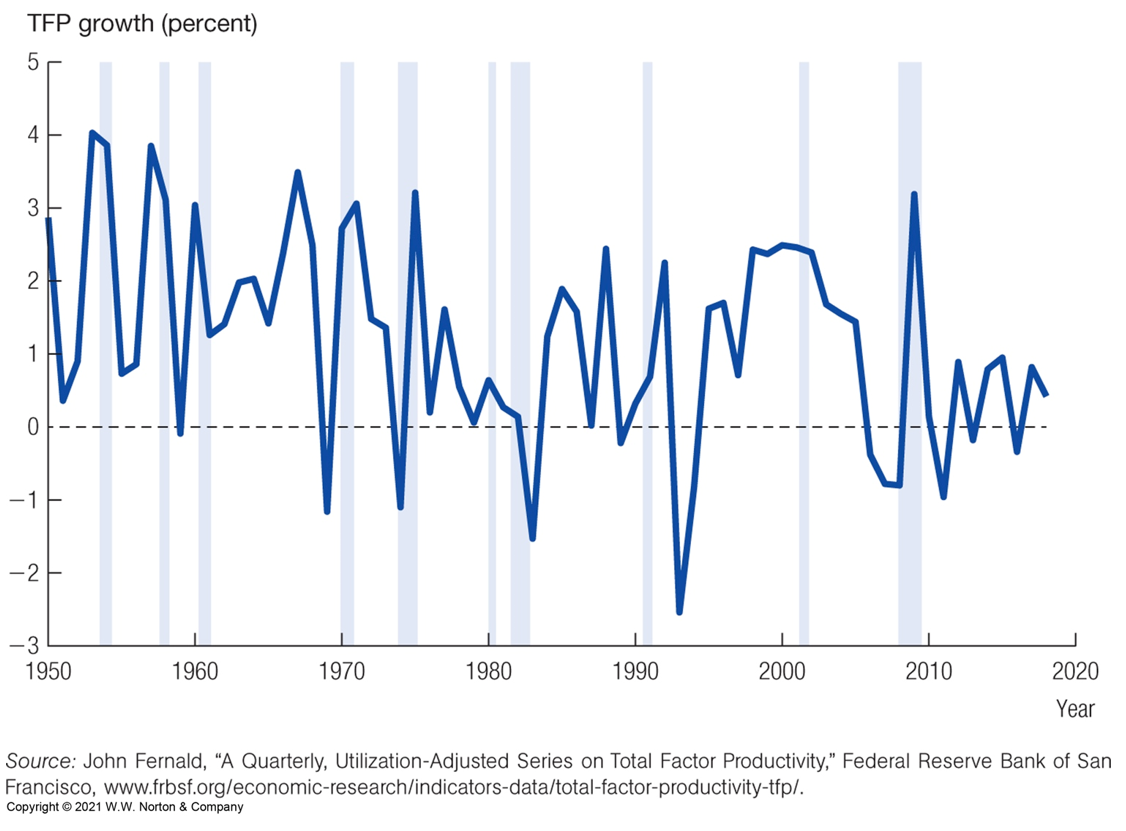
\includegraphics[width=0.7\linewidth]{Figures/fig_15_01}
	\end{figure}
\end{frame}

\begin{frame}[wide]{A Brief History of DSGE Models}
	\begin{itemize}
		\item TFP shocks:
		\begin{itemize}
			\item Positive shocks cause the economy to boom
			\item Negative shocks cause GDP to decline
		\end{itemize}
		\item The economy would go through cycles because of TFP shocks
		\item Shocks to TFP are “real” in RBC and cause output to fluctuate  as in business cycle
		\item Some weaknesses:
		\begin{itemize}
			\item Not all macroeconomic fluctuations are driven by TFP shocks (e.g., 2001)
		\end{itemize}
	\end{itemize}
\end{frame}

\begin{frame}[wide]{From Real Business Cycle to DSGE}
	\begin{itemize}
		\item Nowadays, DSGE models have moved away from the “real” classification by incorporating monetary policy
		\item Components of modern DSGE models
		\begin{itemize}
			\item Endogenous variables
			\item Shocks
			\item Features that affect the way shocks impact endogenous variables over time, for example,
			\begin{itemize}
				\item Various tax (capital, income, etc)
				\item Capital adjustment (firms need time to adjust the level of capital)
				\item Unemployment insurance
			\end{itemize}
		\end{itemize}
		
	\end{itemize}
\end{frame}

\begin{frame}[wide]{Endogenous Variables}
	\begin{itemize}
		\item DSGE models can be large or small systems
		\item One important component of almost all DSGE models is the labour market. Decisions in the labour market determine how much output is produced:
		\begin{itemize}
			\item From the unemployment model we studied, if we want a rich labor market model, we will need Hours worked, Searching for employment, Job effort
		\end{itemize}
		\item Below is a list of potential variables to be included in DSGE:
		\begin{itemize}
			\item wages, interest rates, inflation, hours worked, GDP, consumption, investment, 	government purchases, employment, unemployment, capital, international trade, foreign debt, 	government debt, exchange rates
			
		\end{itemize}
	\end{itemize}
\end{frame}

\begin{frame}[wide]{Shocks}
	\begin{itemize}
		\item Shocks cause endogenous variables to fluctuate
		\begin{itemize}
			\item Include total factor productivity, government purchases, taxes, monetary policy, energy prices, and financial frictions
		\end{itemize}
		\item Shocks can be temporary or permanent
		\begin{itemize}
			\item Some shocks may last only one period. Some shocks may last forever
			\item For instance, government spending may be temporarily high this year, or there could be a long-lasting change in the size of the government
		\end{itemize}
	\end{itemize}
\end{frame}

\begin{frame}[wide]{Shocks}
	\begin{itemize}
		\item Shocks may be current or anticipated
		\begin{itemize}
			\item A shock may occur now or instead we may get news today of a shock that will occur in the future
			\item For example, people anticipate AI would enhance productivity
			\item When news arrive, agent would integrate the news with rational expectation in the decision making
			\item Uncertainty about the future can slow economic activity today as well
		\end{itemize}
	\end{itemize}
\end{frame}

\begin{frame}[wide]{Features and Mathematics}
	\begin{itemize}
		\item DSGE models are complex to solve mathematically because they involve many individual decisions
		\begin{itemize}
			\item DSGE models is calculated using numerical simulations most of the time
		\end{itemize}
		\item Some of the DSGE model's common features:
		\begin{itemize}
			\item Nominal rigidities
			\begin{itemize}
				\item Monetary policy only has real effects if some friction interferes with price adjustment
				\item e.g., Sticky nominal wages and sticky prices
			\end{itemize}
		\end{itemize}
	\end{itemize}
\end{frame}

\begin{frame}[wide]{Features and Mathematics}
	Some of the DSGE model common features:
	\begin{itemize}
		\item Adjustment costs: 
		\begin{itemize}
			\item It is expensive to change the capital stock by a large amount
			\item The dynamic response of variables to shocks is slow to adjust
			\item The effect of the shock occurs several periods after the shock, the opposite of the Solow model, where the effect of the shock is the largest immediately after it hits
		\end{itemize}
	\end{itemize}
\end{frame}

\begin{frame}[wide]{Features and Mathematics}
	Some of the DSGE model common features:
	\begin{itemize}
		\item Incomplete markets:
		\begin{itemize}
			\item Incomplete markets refer to situations where certain financial instruments or contracts are not available to fully hedge against all risks or uncertainties in the economy (i.e., just like in real life)
			\item The early version of economics model assume agent can fully hedge 
			\item In such markets, individuals may constraints to inefficiencies and potentially suboptimal outcomes
			\item Incomplete markets can arise due to factors such as adverse selection, moral hazard, transaction costs, regulatory constraints, or the presence of non-tradable assets, time or geography
			%\item For example, unemployment may be concentrated on a subset of the labour force, and those who are unemployed may experience a disproportionate decline in consumption
		\end{itemize}
	\end{itemize}
\end{frame}

\begin{frame}[wide]{Features and Mathematics}
	Some of the DSGE model common features:
	\begin{itemize}
		\item Heterogeneity: People and firms are different and response to shocks differently
		\begin{itemize}
			\item Some individuals have completely inelastic labour supply, work 40 hours per week or not at all. Meanwhile, some may have the average elastic or very elastic
			\item Also Reservation wage may different across population
			\item When shocks change the wage, people enter and exit from the labour market
			\item The aggregate elasticity depends on the distribution of reservation wages rather than on any individual’s elasticity
			\item When analyzing policy impacts on the population, it would be important to understand which demographic groups will be affected by the policy
			\item The differences between agent can be based on various thing, for example, innate ability, wealth, income, etc
		\end{itemize}
	\end{itemize}
\end{frame}

\begin{frame}[wide]{A Stylized Approach to DSGE}
	\begin{itemize}
		\item Most DSGE models contain at least three markets: Labour, Capital and 	Output
		\item Focus on the labour market here
		\item labour demand: 
		\begin{itemize}
			\item Derived from firm’s profit-maximization problem
			\item Decide how much labour to hire
			\item Negative slope–diminishing MPL
		\end{itemize}
		\item labour supply:
		\begin{itemize}
			\item Decisions by people about how much to work
		\end{itemize}
		
	\end{itemize}
\end{frame}


\begin{frame}[wide]{A Stylized Approach to DSGE: labour Demand}
	\begin{itemize}
		\item The labour demand curve is derived from the firm’s profit maximization problem
		\item Firms hire labour until the MPL equals the wage
		\begin{itemize}
			\item The MPL is dictated by the production function: $Y = AN^\alpha K^{1-\alpha}$
			\item  Marginal product of labour: the amount of extra output produced by the last worker hired
		\end{itemize}
		\item Hire until $MPL= \alpha \frac{A N^\alpha K^{1-\alpha}}{N} = w$
		\item Diminishing marginal returns to labour (exponent less than one) implies that each additional unit of labour that is hired produces a smaller and smaller gain in output
		\item Because of the assumption that the MPL declines as more labour is hired, the labour demand curve is downward sloping
		\item Note here that the TFP shocks ($A$) can directly affecting the MPL
		
	\end{itemize}
\end{frame}

\begin{frame}[wide]{A Stylized Approach to DSGE: labour Supply}
	\begin{itemize}
		\item labour supply is derived from people utility maximization problem with consumption/leisure choice
		\item Use the following specification:  $L^S=\bar{\ell} \frac{w}{c}$
		
		\vspace{1mm}
		where w is the real wage, c denotes consumption per person and $\bar{\ell}$ is the parameter that governs the overall magnitude of labour supply
		
		\item labour supply is increasing in the wage and depends on the wage-to-consumption ratio
		\item Over time, the real wage increases, and consumption per person also rises
		\begin{itemize}
			\item In fact, these growth rates are approximately the same, so that w/c is relatively stable
		\end{itemize}
		\item Therefore, the amount of labour supplied (per person) would be stable as well
	\end{itemize}
\end{frame}

\begin{frame}[wide]{The labour Market in the DSGE Model}
	\begin{itemize}
		\item The equilibrium determines the real wage and the amount of labour that gets used in production
	\end{itemize}
	\begin{figure}
		\centering
		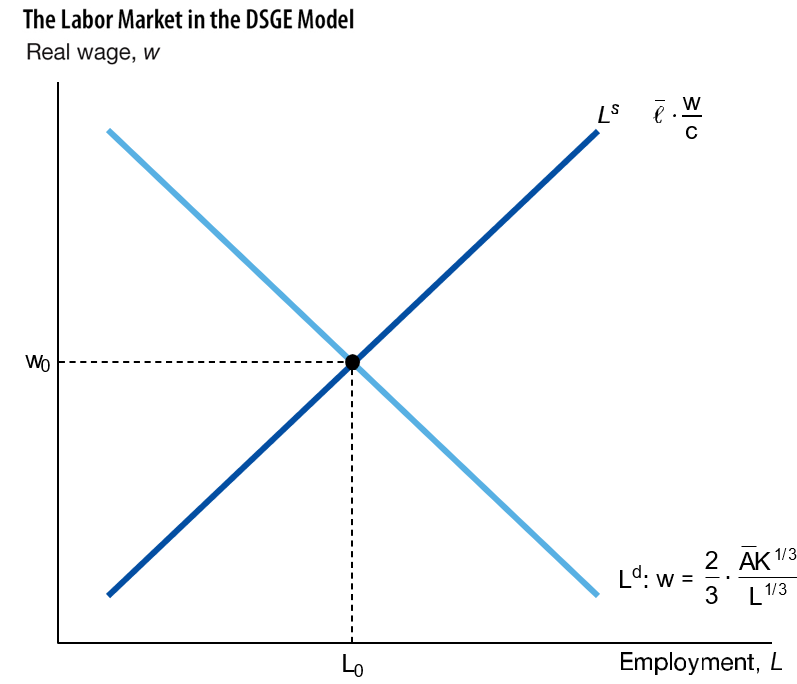
\includegraphics[width=0.5\linewidth]{Figures/fig_15_02}
	\end{figure}
	
\end{frame}

\begin{frame}[wide]{Using the Stylized DSGE Model}
	Examine the following:
	\begin{itemize}
		\item a TFP shock 
		\item a change in taxes 
		\item a rise in the size of  government purchases
		\item a shock to monetary policy
		
	\end{itemize}
\end{frame}

\begin{frame}[wide]{A Negative TFP Shock in the DSGE Model}
	\begin{itemize}
		\item A temporarily negative shock that reduces the TFP parameter
		\begin{itemize}
			\item Lower A decreases the amount of output that an extra worker can produce.
			\item The MPL is lower for any given L
		\end{itemize}
		\item Firms do not want to produce due to low demand, so labour demand shifts down
		\item The TFP shock is temporary, so effects on consumption are small (i.e., no shift on labour supply curve)
		\item In response to a negative TFP shock, employment falls, and the equilibrium wage falls 
		\begin{itemize}
			\item A nice result that would match business cycle fact, lead the early DSGE models to focus on TFP shocks
		\end{itemize}
	\end{itemize}
\end{frame}

\begin{frame}[wide]{A Negative TFP Shock in the DSGE Model}
	\begin{figure}
		\centering
		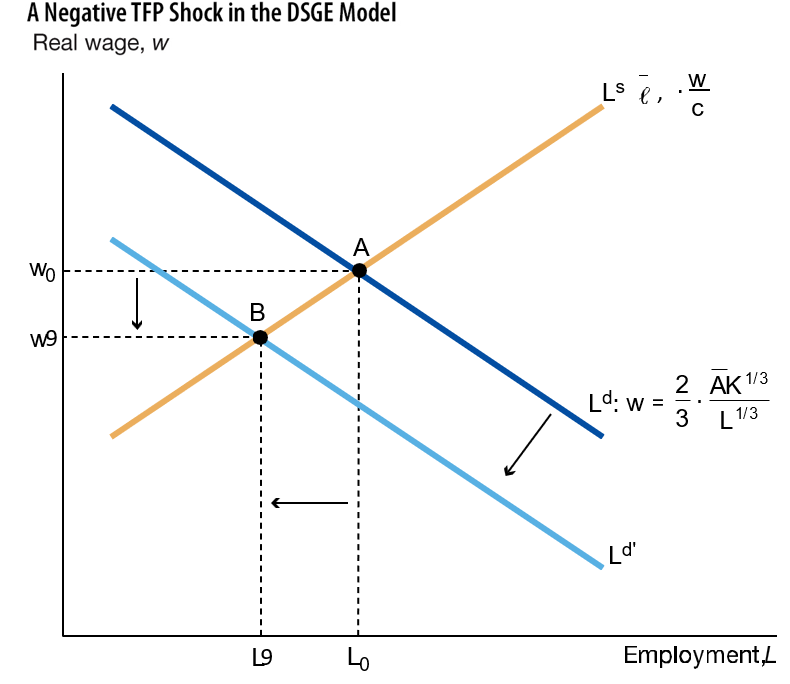
\includegraphics[width=0.5\linewidth]{Figures/fig_15_03}
	\end{figure}
	
\end{frame}

\begin{frame}[wide]{The Imposition of a Sales Tax in the DSGE Model}
	\begin{itemize}
		\item Suppose firms must pay a tax for every dollar of output they sell temporarily
		\item Since firms pay the tax, the labour demand curve shifts
		\begin{itemize}
			\item This reduces the amount that the firm earns at any given level of employment, lowering the MPL and shifting the labour demand curve in
		\end{itemize}
		\item Firms now hire until the after-tax marginal product of labour falls to equal the wage
		\[(1-t) \alpha \frac{Y}{N} = w\]
		\item There are no effect on consumption. Once again, no shift on the labour supply curve
	\end{itemize}
\end{frame}

\begin{frame}[wide]{The Imposition of a Sales Tax in the DSGE Model}
	\begin{itemize}
		\item Wages and employment decline
	\end{itemize}
	\begin{figure}
		\centering
		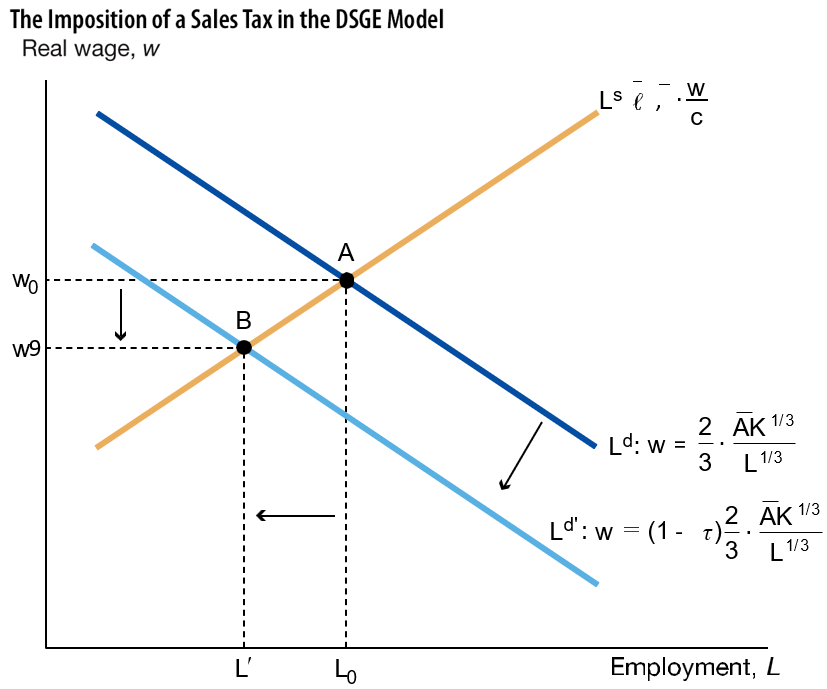
\includegraphics[width=0.6\linewidth]{Figures/fig_15_04}
	\end{figure}
\end{frame}

\begin{frame}[wide]{A Rise in Government Purchases}
	\begin{itemize}
		\item Consider an increase in government purchases, financed through a rise in lump-sum taxes at some unspecified point in the future
		\item The implied tax burden lowers permanent income and therefore reduces consumption today
		\begin{itemize}
			\item Consumption is the variable in our DSGE model that allows future events to affect the economy today
		\end{itemize}
		\item A general principle in microeconomics is that as people get richer, they generally consume more of all goods, including leisure
		\begin{itemize}
			\item This means that consumption and leisure will typically move in the same direction
			\item This means the labour supply curve shifts to the right
		\end{itemize}
		\item There are no change to labour demand curve this time
	\end{itemize}
\end{frame}

\begin{frame}[wide]{A Rise in Government Purchases}
	\begin{itemize}
		\item The equilibrium effect of this shock is to increase employment and reduce the real wage
	\end{itemize}
	\begin{figure}
		\centering
		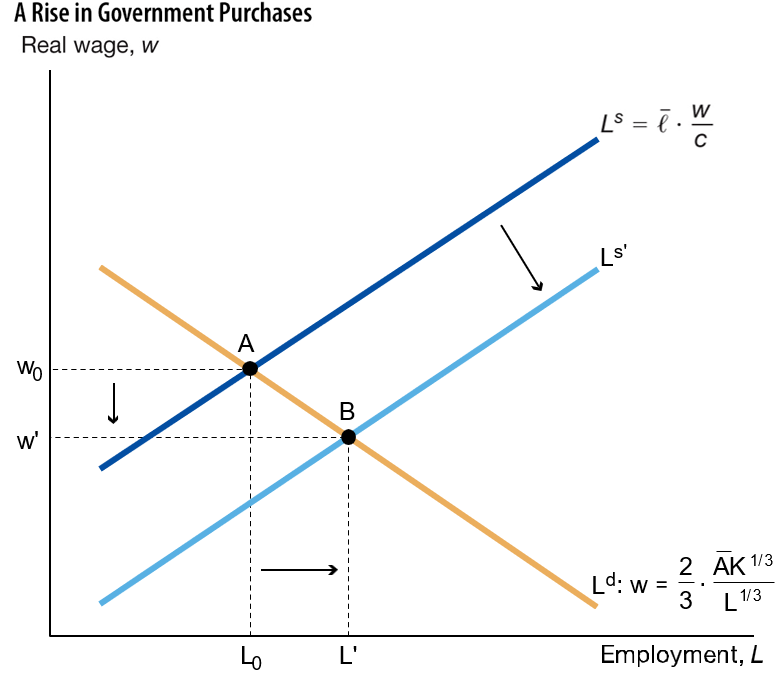
\includegraphics[width=0.5\linewidth]{Figures/fig_15_05}
	\end{figure}
	
\end{frame}

\begin{frame}[wide]{Sticky Wages}
	\begin{itemize}
		
		\item For monetary policy to have real effects on the economy, we must introduce frictions in the adjustment of prices
		\begin{itemize}
			\item If the classical dichotomy holds, changes in monetary policy does not have any effect on real variables
		\end{itemize}
		\item Distinguish between nominal and real variables
		\begin{itemize}
			\item W is the nominal wage
			\item P is the price level
			\item W/P = w is the real wage 
		\end{itemize}
	\end{itemize}
\end{frame}

\begin{frame}[wide]{Sticky Wages in the DSGE Model}
	\begin{itemize}
		\item Under sticky wages, the wage does not adjust when the market condition change
		\[W = \bar{W}\]
		\item Employment is set by the demand side in this case, as both sides of the trade must be willing participants -- take the one with lower employment level
	\end{itemize}
	\begin{figure}
		\centering
		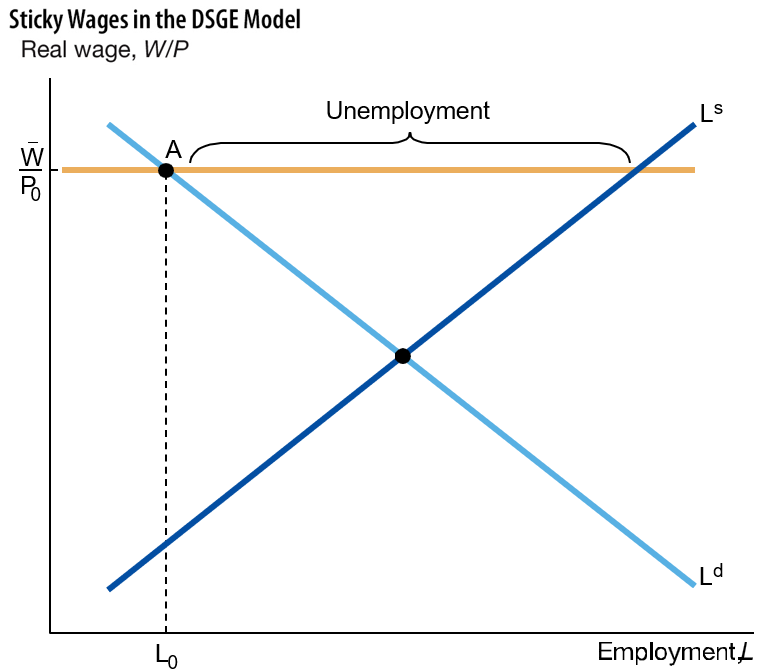
\includegraphics[width=0.45\linewidth]{Figures/fig_15_06}
	\end{figure}
\end{frame}

\begin{frame}[wide]{A Monetary Expansion with Sticky Wages}
	\begin{itemize}
		\item When there is expansionary monetary policy, lowering the federal funds rate increases other prices  (like in our AD curve)
		\begin{itemize}
			\item But wages are still sticky
		\end{itemize}
		\item The overall price level P rises to some new level P’
		\item With the nominal wage stuck at W, the price increase leads the real wage W/P to decline
		\item The equilibrium is then move down along the demand curve
	\end{itemize}
\end{frame}

\begin{frame}[wide]{A Monetary Expansion with Sticky Wages}
	\begin{itemize}
		\item At this lower real wage, labour demand is higher and labour supply is lower
		\item This is not the signature pattern we would expect. Real wages are generally low during Booms
	\end{itemize}
	\begin{figure}
		\centering
		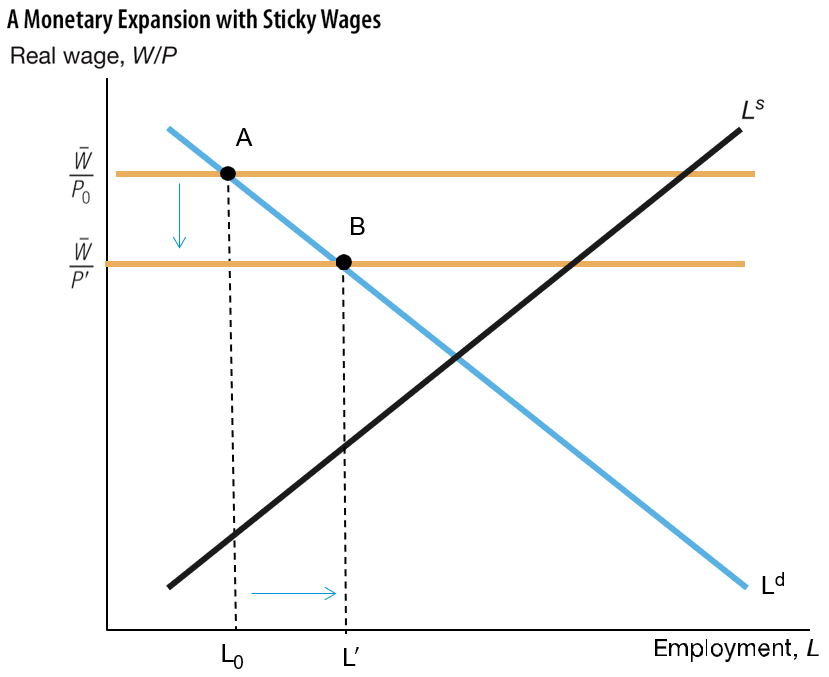
\includegraphics[width=0.5\linewidth]{Figures/fig_15_07}
	\end{figure}
	
\end{frame}

\begin{frame}[wide]{A Monetary Expansion with Sticky Prices}
	\begin{itemize}
		\item In the Keynesian tradition, the output is determined by the demand
		\begin{itemize}
			\item Firms must demand the amount of labour that is needed to produce the demanded output
			\item In this case, the labor demand curve is now vertical
		\end{itemize} 
		\item Consider the effect of an expansionary monetary policy (a lower fed funds rate) under sticky prices (i.e., $P=\bar{P}$ instead of wages)
		\item The monetary expansion increases demand in the economy since prices are fixed
		\item Firms need to produce a higher level of output and therefore require more labor: the labor demand curve shifts to the right
	\end{itemize}
\end{frame}

\begin{frame}[wide]{A Monetary Expansion with Sticky Prices}
	\begin{itemize}
		\item To induce more people to work, the wage must rise (recall that the nominal wage is flexible in this case), and with sticky prices, this leads to an increase in real wages, as the economy moves to point B
	\end{itemize}
	\begin{figure}
		\centering
		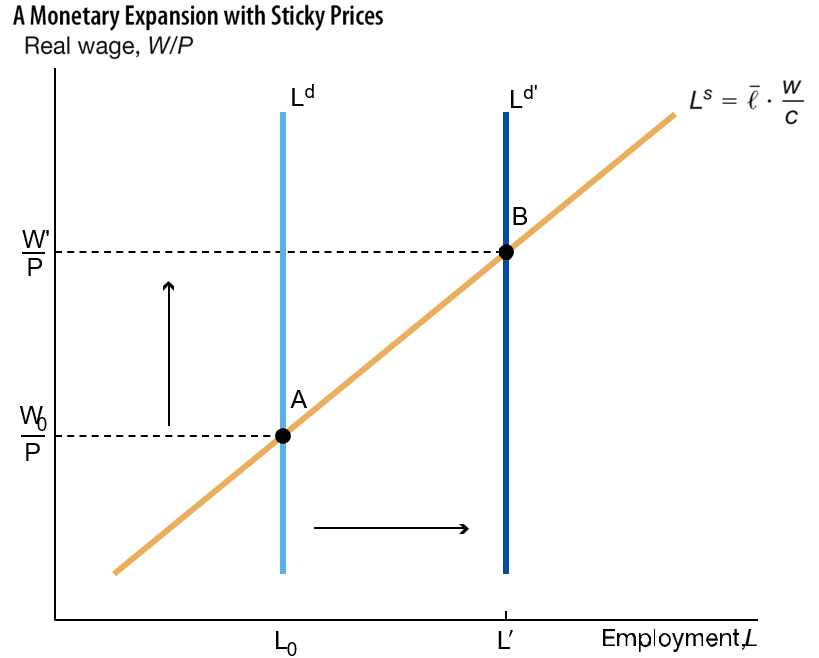
\includegraphics[width=0.45\linewidth]{Figures/fig_15_08}
	\end{figure}
	
\end{frame}

%\begin{frame}[wide]{An Increase in the Investment Rate}
%	\begin{columns} 
%			% Column 1
%			\begin{column}{.5\textwidth}
%				\begin{itemize}
%					\item Suppose the investment rate increases permanently for exogenous reasons ($s'>s$)
%					\begin{itemize}
%						\item The investment curve rotates upward ($\bar{s}'\bar{A}  \bar{L}^{1-\alpha} K_t^\alpha > \bar{s}\bar{A}  \bar{L}^{1-\alpha} K_t^\alpha$)
%						\item The depreciation curve remains unchanged ($\delta K_t$)
%						\item The capital stock increases by transition dynamics to reach the new steady state
%						\begin{itemize}
%							\item This happens because investment exceeds depreciation ($sY_t>\delta K_t$)
%						\end{itemize}
%						\item The new steady state is located to the right
%					\end{itemize}
%				\end{itemize}
%			\end{column}
%			% Column 2    
%			\begin{column}{.5\textwidth}			
%				\begin{figure}
%					\centering
%					\includegraphics[width=1\linewidth]{"Figures/An Increase in the Investment Rate"}
%				\end{figure}
%			\end{column}%
%		\end{columns}
%\end{frame}

%\begin{frame}[wide]{Measuring the State of the Economy}
%	\begin{columns} 
%		% Column 1
%		\begin{column}{.5\textwidth}
%			\begin{table}[htbp]
%				\centering
%				\begin{tabular}{lrrrr}
%					& 2005  & 2006  & 2007  & 2008 \\
%					\hline
%					GDP   & 12.6  & 13.4  & 14.0    & 14.3 \\
%					(in trillions of \$) &       &       &       &  \\
%					Growth rate GDP &       & 0.063 & 0.045 & 0.021 \\
%					\hline
%				\end{tabular}%
%				\label{tab:addlabel}%
%			\end{table}%
%		\end{column}
%		% Column 2    
%		\begin{column}{.5\textwidth}			
%			
%			
%		\end{column}%
%	\end{columns}
%\end{frame}

\begin{frame}[wide]{Next Lecture}
	\begin{itemize}
		\item Next lecture will finish Ch. 15 and begin Ch. 18
	\end{itemize}
\end{frame}

\end{document}